\documentclass{article}
\usepackage{tikz}
\usetikzlibrary{trees}

\begin{document}

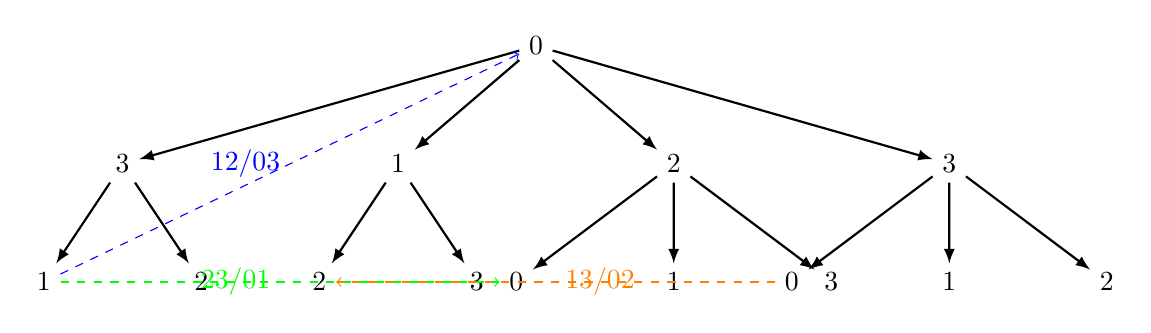
\begin{tikzpicture}[level distance=1.5cm,
  level 1/.style={sibling distance=3.5cm},
  level 2/.style={sibling distance=2cm},
  level 3/.style={sibling distance=1.5cm},
  edge from parent/.style={draw,thick,-latex}]

\node (root) {0}
    child {node {3}
        child {node {1}}
        child {node {2}}}
    child {node {1}
        child {node {2}}
        child {node {3}}}
    child {node {2}
        child {node {0}}
        child {node {1}}
        child {node {3}}}
    child {node {3}
        child {node {0}}
        child {node {1}}
        child {node {2}}};

% Arrows and labels
\draw[blue, dashed, ->] (root-1-1) -- node[left] {$12/03$} (root);
\draw[orange, dashed, ->] (root-4-1) -- node[right] {$13/02$} (root-2-1);
\draw[green, dashed, ->] (root-1-1) -- node[left] {$23/01$} (root-3-1);

\end{tikzpicture}

\end{document}